\subsection{xVertSeg}

The xVertSeg \cite{Ibragimov2012, xxx} was kindly made available by prof. T. Vrtovec (University of Ljubljana, Faculty of Electrical Engineering, Slovenia), see appendix \ref{seg:datasetagreement} for the agreement.
This dataset contains 25 \acrfull{ct} scans of the lumbar spine, of which 15 \acrshort{ct} scans are fully labeled.
Given the provided data, I can assume these 15 scans were collected from 15 different patients.

For each of these 15 scans, full instance segmenation masks for all 5 lumbar vertebrae are provided. The delineation was performed by a skilled professional.

Additionally, for each vertebra a fracture class and fracture grade is provided. 
Apart from vertebrae classified as \textit{normal}, the dataset contains \textit{mild}, \textit{moderate} and \textit{severe} cases of vertebrae fracture types \textit{wedge}, \textit{crush} and \textit{biconcavity}.
\marginpar{
        % This file was created by tikzplotlib v0.9.8.
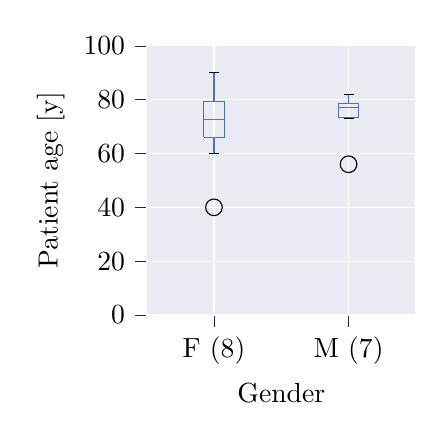
\begin{tikzpicture}

\definecolor{color0}{rgb}{0.917647058823529,0.917647058823529,0.949019607843137}
\definecolor{color1}{rgb}{0.298039215686275,0.447058823529412,0.690196078431373}
\definecolor{color2}{rgb}{0.768627450980392,0.305882352941176,0.32156862745098}

\begin{axis}[
axis background/.style={fill=color0},
axis line style={white},
height=5cm,
tick align=outside,
tick pos=left,
width=5cm,
x grid style={white},
xlabel={Gender},
xmajorgrids,
xmin=0.5, xmax=2.5,
xtick style={color=white!15!black},
xtick={1,2},
xticklabels={F (8),M (7)},
y grid style={white},
ylabel={Patient age [y]},
ymajorgrids,
ymin=0, ymax=100,
ytick style={color=white!15!black}
]
\addplot [color1, opacity=1]
table {%
0.925 66
1.075 66
1.075 79.25
0.925 79.25
0.925 66
};
\addplot [color1, opacity=1]
table {%
1 66
1 60
};
\addplot [color1, opacity=1]
table {%
1 79.25
1 90
};
\addplot [black, opacity=1]
table {%
0.9625 60
1.0375 60
};
\addplot [black, opacity=1]
table {%
0.9625 90
1.0375 90
};
\addplot [black, mark=o, mark size=3, mark options={solid,fill opacity=0}, only marks]
table {%
1 40
};
\addplot [color1, opacity=1]
table {%
1.925 73.5
2.075 73.5
2.075 78.5
1.925 78.5
1.925 73.5
};
\addplot [color1, opacity=1]
table {%
2 73.5
2 73
};
\addplot [color1, opacity=1]
table {%
2 78.5
2 82
};
\addplot [black, opacity=1]
table {%
1.9625 73
2.0375 73
};
\addplot [black, opacity=1]
table {%
1.9625 82
2.0375 82
};
\addplot [black, mark=o, mark size=3, mark options={solid,fill opacity=0}, only marks]
table {%
2 56
};
\addplot [color2, opacity=1]
table {%
0.925 72.5
1.075 72.5
};
\addplot [color2, opacity=1]
table {%
1.925 77
2.075 77
};
\end{axis}

\end{tikzpicture}

        \captionof{figure}{xVertSeg patients age distribution}
        \label{fig:xVertSeg_Age}
    }

\subsubsection{Original Objective of the Dataset}

The objective of the \textit{xVertSeg challenge}\footnote{see \url{http://lit.fe.uni-lj.si/xVertSeg/database.php}} (2015) was organized by the University of Ljubljana.
Based on the 15 provided scans with corresponding masks, the participans were required to construct a model to make predictions on the test set of 10 unlabelled scans.

The challenge consisted of two tasks:
\begin{enumerate}
    \item Segmentation of the lumbar vertebrae. For each scan in the test set, the segmentation masks of the lumbar vertebrae were requested.
    \item Fracture classification on the segmented vertebrae, consisting of morphological grade and fracture classification.
\end{enumerate}

\subsubsection{Patient statistics}

The patients in the xVertSeg dataset train set consist of 8 females and 7 males.
The age of these patients is slightly higher than for the other datasets.
The average patient in this dataset is 71 years old.
A box plot of the age distribution between genders is shown in figure \ref{fig:xVertSeg_Age}. 

\begin{SCtable}[\sidecaptionrelwidth][h]
    \centering
        \begin{tabular}{lrrrrrr}
\toprule
{} &  L1 &  L2 &  L3 &  L4 &  L5 &  Total \\
\midrule
biconcave &   6 &   7 &   8 &   4 &   2 &     27 \\
normal    &   5 &   6 &   4 &   4 &   7 &     26 \\
wedge     &   3 &   2 &   2 &   3 &   2 &     12 \\
crush     &   1 &   0 &   1 &   4 &   4 &     10 \\
\bottomrule
\end{tabular}

        \caption{Every patient in the xVertSeg dataset suffers from at least one spine pathology.
        Most of these pathologies are identified as \textit{mild}.
        This table counts the spine pathologies and normal vertebrae observed over all 15 patients in the xVertSeg dataset.}   
\end{SCtable}

\subsubsection{Technical information}

The xVertSeg dataset contains 15 \acrshort{ct} annotated scans. 
This dataset is very interesting due to the high quality and high resolution of the images.
On figure \ref{fig:xVertSeg_image002}, two slices of the same patient (002) are represented.
The slices show the complete, uncropped sections of the torso and abdominal region of the patient. 
There is no \acrshort{roi} cropping.

\begin{SCfigure}[][htb]
    \centering
    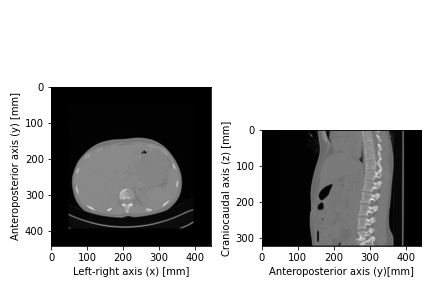
\includegraphics[width=.95\textwidth]{automated_graphs/xVertSeg_image002.png}
    \caption{xVertSeg scan \textit{image002}. \label{fig:xVertSeg_image002}}
\end{SCfigure}

The distribution of the scan dimensions is shown in figure \ref{fig:AllDataset_dims}. This also illustrates the \textit{xVertSeg} dataset consists of large, high resolution images.
Mind that during pre-processing the scans are resampled on a $1mm \times 1mm \times 1mm$ grid.